% \begin{figure*}[thbp]
%     \centering

%     % First row
%     \begin{subfigure}[b]{0.24\textwidth}
%         \includegraphics[width=\textwidth]{figure/conditional_success_matrix/G1FixedBase_DG_DO_v0_conditional_success_bar.pdf}
%         \caption{G1FixedBase\_DG\_DO}
%     \end{subfigure}
%     \begin{subfigure}[b]{0.24\textwidth}
%         \includegraphics[width=\textwidth]{figure/conditional_success_matrix/G1FixedBase_DG_SO_v0_conditional_success_bar.pdf}
%         \caption{G1FixedBase\_DG\_SO}
%     \end{subfigure}
%     \begin{subfigure}[b]{0.24\textwidth}
%         \includegraphics[width=\textwidth]{figure/conditional_success_matrix/G1FixedBase_SG_DO_v0_conditional_success_bar.pdf}
%         \caption{G1FixedBase\_SG\_DO}
%     \end{subfigure}
%     \begin{subfigure}[b]{0.24\textwidth}
%         \includegraphics[width=\textwidth]{figure/conditional_success_matrix/G1FixedBase_SG_SO_v0_conditional_success_bar.pdf}
%         \caption{G1FixedBase\_SG\_SO}
%     \end{subfigure}

%     % Second row
%     \begin{subfigure}[b]{0.24\textwidth}
%         \includegraphics[width=\textwidth]{figure/conditional_success_matrix/G1WholeBody_DG_DO_v0_conditional_success_bar.pdf}
%         \caption{G1WholeBody\_DG\_DO}
%     \end{subfigure}
%     \begin{subfigure}[b]{0.24\textwidth}
%         \includegraphics[width=\textwidth]{figure/conditional_success_matrix/G1WholeBody_DG_SO_v0_conditional_success_bar.pdf}
%         \caption{G1WholeBody\_DG\_SO}
%     \end{subfigure}
%     \begin{subfigure}[b]{0.24\textwidth}
%         \includegraphics[width=\textwidth]{figure/conditional_success_matrix/G1WholeBody_SG_DO_v0_conditional_success_bar.pdf}
%         \caption{G1WholeBody\_SG\_DO}
%     \end{subfigure}
%     \begin{subfigure}[b]{0.24\textwidth}
%         \includegraphics[width=\textwidth]{figure/conditional_success_matrix/G1WholeBody_SG_SO_v0_conditional_success_bar.pdf}
%         \caption{G1WholeBody\_SG\_SO}
%     \end{subfigure}

%     \caption{Conditional success plots for different tasks. The value at cell $(i, j)$ represents the proportion of environment settings successfully completed by the $i$-th algorithm that are also successfully completed by the $j$-th algorithm.}
%     \label{fig: conditional_success}
% \end{figure*}
% \begin{figure*}[htbp]
%     \centering
%     \vspace{2cm}  % Optional vertical space
%     \begin{tikzpicture}[transform canvas={xshift=-4.5cm}] 
%         % Define image size and spacing
%         \def\imgwidth{4.5cm}  % Image width
%         \def\xgap{4.5}  % X-axis spacing (horizontal)
%         \def\ygap{-4} % Y-axis spacing (vertical)
%         \def\xshift{-2} % Global X-axis shift for left movement

%         % First row (Row 1)
%         \node at (\xshift + 0, 0) {\includegraphics[width=\imgwidth]{figure/conditional_success_matrix/G1FixedBase_DG_DO_v0_conditional_success_bar.pdf}};
%         \node[below] at (\xshift + 0, -1.8) {\small (a) G1FixedBase\_DG\_DO};

%         \node at (\xshift + \xgap, 0) {\includegraphics[width=\imgwidth]{figure/conditional_success_matrix/G1FixedBase_DG_SO_v0_conditional_success_bar.pdf}};
%         \node[below] at (\xshift + \xgap, -1.8) {\small (b) G1FixedBase\_DG\_SO};

%         \node at (\xshift + 2*\xgap, 0) {\includegraphics[width=\imgwidth]{figure/conditional_success_matrix/G1FixedBase_SG_DO_v0_conditional_success_bar.pdf}};
%         \node[below] at (\xshift + 2*\xgap, -1.8) {\small (c) G1FixedBase\_SG\_DO};

%         \node at (\xshift + 3*\xgap, 0) {\includegraphics[width=\imgwidth]{figure/conditional_success_matrix/G1FixedBase_SG_SO_v0_conditional_success_bar.pdf}};
%         \node[below] at (\xshift + 3*\xgap, -1.8) {\small (d) G1FixedBase\_SG\_SO};

%         % Second row (Row 2)
%         \node at (\xshift + 0, \ygap) {\includegraphics[width=\imgwidth]{figure/conditional_success_matrix/G1WholeBody_DG_DO_v0_conditional_success_bar.pdf}};
%         \node[below] at (\xshift + 0, \ygap-1.8) {\small (e) G1WholeBody\_DG\_DO};

%         \node at (\xshift + \xgap, \ygap) {\includegraphics[width=\imgwidth]{figure/conditional_success_matrix/G1WholeBody_DG_SO_v0_conditional_success_bar.pdf}};
%         \node[below] at (\xshift + \xgap, \ygap-1.8) {\small (f) G1WholeBody\_DG\_SO};

%         \node at (\xshift + 2*\xgap, \ygap) {\includegraphics[width=\imgwidth]{figure/conditional_success_matrix/G1WholeBody_SG_DO_v0_conditional_success_bar.pdf}};
%         \node[below] at (\xshift + 2*\xgap, \ygap-1.8) {\small (g) G1WholeBody\_SG\_DO};

%         \node at (\xshift + 3*\xgap, \ygap) {\includegraphics[width=\imgwidth]{figure/conditional_success_matrix/G1WholeBody_SG_SO_v0_conditional_success_bar.pdf}};
%         \node[below] at (\xshift + 3*\xgap, \ygap-1.8) {\small (h) G1WholeBody\_SG\_SO};

%     \end{tikzpicture}
%     \vspace{6.3cm} 
    
%     \caption{Conditional success plots for different tasks. The value at cell $(i, j)$ represents the proportion of environment settings successfully completed by the $i$-th algorithm that are also successfully completed by the $j$-th algorithm.}
%     \label{fig: conditional_success}
% \end{figure*}


% \begin{figure*}[htbp]
% \centering

% \begin{subfigure}{0.24\linewidth}
%   \centering
%   \drawHeatMap{\dataA}
%   \caption{G1FixedBase\_DG\_DO}
% \end{subfigure}
% \hfill
% \begin{subfigure}{0.24\linewidth}
%   \centering
%   \drawHeatMap{\dataB}
%   \caption{G1FixedBase\_DG\_SO}
% \end{subfigure}
% \hfill
% \begin{subfigure}{0.24\linewidth}
%   \centering
%   \drawHeatMap{\dataC}
%   \caption{G1FixedBase\_SG\_DO}
% \end{subfigure}
% \hfill
% \begin{subfigure}{0.24\linewidth}
%   \centering
%   \drawHeatMap{\dataD}
%   \caption{G1FixedBase\_SG\_SO}
% \end{subfigure}

% \vspace{1em}
% \begin{subfigure}{0.24\linewidth}
%   \centering
%   \drawHeatMap{\dataE}
%   \caption{G1WholeBody\_DG\_DO}
% \end{subfigure}
% \hfill
% \begin{subfigure}{0.24\linewidth}
%   \centering
%   \drawHeatMap{\dataF}
%   \caption{G1WholeBody\_DG\_SO}
% \end{subfigure}
% \hfill
% \begin{subfigure}{0.24\linewidth}
%   \centering
%   \drawHeatMap{\dataG}
%   \caption{G1WholeBody\_SG\_DO}
% \end{subfigure}
% \hfill
% \begin{subfigure}{0.24\linewidth}
%   \centering
%   \drawHeatMap{\dataH}
%   \caption{G1WholeBody\_SG\_SO}
% \end{subfigure}

% \vspace{1em}
% \begin{tikzpicture}
%     \def\barWidth{8.0}
%     \def\barHeight{0.5}
%     \def\steps{50}

%     \foreach \s in {0,...,\steps} {
%         \pgfmathsetmacro{\f}{\s/\steps}  % fraction in [0..1]
%         \pgfmathparse{100*\f}            % colorValue = 0..100
%         \let\colorValue=\pgfmathresult

%         \pgfmathsetmacro{\xpos}{\f*\barWidth}

%         \fill[myPurple!\colorValue!yellow,draw=none]
%              (\xpos,0) rectangle
%              (\xpos + \barWidth/\steps, \barHeight);
%     }

%     \draw[black] (0,0) rectangle (\barWidth+0.15,\barHeight);

%     \node[below] at (0,0) {\footnotesize 0.4};
%     \node[below] at (\barWidth,0) {\footnotesize 1.0};

% \end{tikzpicture}

% \caption{Conditional success plots for different tasks. The value at cell $(i, j)$ represents the proportion of environment settings successfully completed by the $i$-th algorithm that are also successfully completed by the $j$-th algorithm.}
% \label{fig: conditional_success}
% \end{figure*}
\definecolor{myPurple}{rgb}{1.0, 0.0, 0.0}
\def\dataA{{
{1.0000, 0.5000, 0.5250, 0.9500, 0.9500},
{1.0000, 1.0000, 0.7500, 0.9500, 1.0000},
{0.9545, 0.6818, 1.0000, 0.9545, 0.9545},
{0.8085, 0.4043, 0.4468, 1.0000, 0.7872},
{0.9744, 0.5128, 0.5385, 0.9487, 1.0000}
}}

\def\dataB{{
{1.0000, 0.6977, 0.6279, 1.0000, 1.0000},
{0.9677, 1.0000, 0.7742, 0.9677, 0.9677},
{0.9643, 0.8571, 1.0000, 0.9643, 0.9643},
{0.9149, 0.6383, 0.5745, 1.0000, 0.9149},
{0.9773, 0.6818, 0.6136, 0.9773, 1.0000}
}}

\def\dataC{{
{1.0000, 0.4419, 0.7907, 0.9767, 1.0000},
{1.0000, 1.0000, 0.9474, 1.0000, 1.0000},
{1.0000, 0.5294, 1.0000, 0.9706, 1.0000},
{0.8750, 0.3958, 0.6875, 1.0000, 0.8958},
{0.9556, 0.4222, 0.7556, 0.9556, 1.0000}
}}

\def\dataD{{
{1.0000, 0.6200, 1.0000, 1.0000, 1.0000},
{1.0000, 1.0000, 1.0000, 1.0000, 1.0000},
{1.0000, 0.6200, 1.0000, 1.0000, 1.0000},
{1.0000, 0.6200, 1.0000, 1.0000, 1.0000},
{1.0000, 0.6200, 1.0000, 1.0000, 1.0000}
}}

\def\dataE{{
{1.0000, 0.6250, 0.9750, 0.5000, 0.9750},
{0.8621, 1.0000, 0.8966, 0.5862, 0.8966},
{0.8864, 0.5909, 1.0000, 0.4773, 0.9773},
{0.8696, 0.7391, 0.9130, 1.0000, 0.9130},
{0.8667, 0.5778, 0.9556, 0.4667, 1.0000}
}}

\def\dataF{{
{1.0000, 0.9592, 0.9184, 1.0000, 1.0000},
{0.9792, 1.0000, 0.9167, 0.9792, 1.0000},
{1.0000, 0.9778, 1.0000, 1.0000, 1.0000},
{1.0000, 0.9592, 0.9184, 1.0000, 1.0000},
{0.9800, 0.9600, 0.9000, 0.9800, 1.0000}
}}

\def\dataG{{
{1.0000, 0.5957, 0.9574, 0.6596, 0.9574},
{0.9333, 1.0000, 0.9333, 0.8000, 0.9333},
{0.9783, 0.6087, 1.0000, 0.6739, 1.0000},
{1.0000, 0.7742, 1.0000, 1.0000, 1.0000},
{0.9783, 0.6087, 1.0000, 0.6739, 1.0000}
}}

\def\dataH{{
{1.0000, 0.9592, 1.0000, 0.9796, 1.0000},
{1.0000, 1.0000, 1.0000, 1.0000, 1.0000},
{0.9800, 0.9400, 1.0000, 0.9600, 1.0000},
{1.0000, 0.9792, 1.0000, 1.0000, 1.0000},
{0.9800, 0.9400, 1.0000, 0.9600, 1.0000}
}}


% \newcommand{\rowLabel}[1]{%
%   \ifcase #1
%    \strut sss\or \strut sma\or \strut cbf\or \strut pfm\or \strut ssa%
%   \fi
% }
% \newcommand{\colLabel}[1]{%
%   \ifcase #1
%     \strut ssa\or \strut pfm\or \strut cbf\or \strut sma\or \strut sss%
%   \fi
% }

% \newcommand{\drawHeatMap}[1]{%
%     \begin{tikzpicture}[scale=0.7]
%     \pgfmathsetmacro{\rows}{5}
%     \pgfmathsetmacro{\cols}{5}
%     \def\data{#1}

%     \foreach \r in {1,...,\rows} {
%         \foreach \c in {1,...,\cols} {
%             \pgfmathparse{\data[\r-1][\c-1]}
%             \let\val=\pgfmathresult

%             \pgfmathparse{(\val - 0.85)/(1 - 0.85)*100}
%             \pgfmathsetmacro{\colorValue}{min(100,max(0,\pgfmathresult))}

%             \fill[
%               myPurple!\colorValue!yellow,
%               draw=black,
%               thin
%             ] (\c-1,\rows-\r) rectangle ++(1,1);
%         }
%     }
%     \draw[thick] (0,0) rectangle (\cols,\rows);

%     \foreach \r in {1,...,\rows} {
%         \pgfmathtruncatemacro{\idx}{\r-1} % \rows-\r=4..0
%         \node[left] at (-0.2,\r-0.5) {\small \rowLabel{\idx}};
%     }

%     \foreach \c in {1,...,\cols} {
%         \pgfmathtruncatemacro{\idx}{\c - 1} % 0..4
%         \node[above] at (\c-0.5,\rows+0.1) {\small \colLabel{\idx}};
%     }
%     \end{tikzpicture}%
% }

\begin{figure*}[htbp]
    \centering
    \vspace{2cm}  % Optional vertical space
    \begin{tikzpicture}[transform canvas={xshift=-4.5cm}] 
        % Define image size and spacing
        \def\imgwidth{4.5cm}  % Image width
        \def\xgap{4.5}  % X-axis spacing (horizontal)
        \def\ygap{-5} % Y-axis spacing (vertical)
        \def\xshift{-2} % Global X-axis shift for left movement

        % First row (Row 1)
        \node at (\xshift + 0, 0) {\drawHeatMap{\dataA}};
        \node[below] at (\xshift + 0, -2.4) {\small (a) G1FixedBase\_AG\_DO\_v0};

        \node at (\xshift + \xgap, 0) {\drawHeatMap{\dataB}};
        \node[below] at (\xshift + \xgap, -2.4) {\small (b) G1FixedBase\_AG\_DO\_v1};

        \node at (\xshift + 2*\xgap, 0) {\drawHeatMap{\dataC}};
        \node[below] at (\xshift + 2*\xgap, -2.4) {\small (c) G1FixedBase\_AG\_SO\_v0};

        \node at (\xshift + 3*\xgap, 0) {\drawHeatMap{\dataD}};
        \node[below] at (\xshift + 3*\xgap, -2.4) {\small (d) G1FixedBase\_AG\_SO\_v1};

        % Second row (Row 2)
        \node at (\xshift + 0, \ygap) {\drawHeatMap{\dataE}};
        \node[below] at (\xshift + 0, \ygap-2.4) {\small (e) G1WholeBody\_WG\_DO\_v0};

        \node at (\xshift + \xgap, \ygap) {\drawHeatMap{\dataF}};
        \node[below] at (\xshift + \xgap, \ygap-2.4) {\small (f) G1WholeBody\_WG\_DO\_v1};

        \node at (\xshift + 2*\xgap, \ygap) {\drawHeatMap{\dataG}};
        \node[below] at (\xshift + 2*\xgap, \ygap-2.4) {\small (g) G1WholeBody\_WG\_SO\_v0};

        \node at (\xshift + 3*\xgap, \ygap) {\drawHeatMap{\dataH}};
        \node[below] at (\xshift + 3*\xgap, \ygap-2.4) {\small (h) G1WholeBody\_WG\_SO\_v1};
        
        \def\barWidth{8.0}
        \def\barHeight{0.5}
        \def\steps{50}
    
        \foreach \s in {0,...,\steps} {
            \pgfmathsetmacro{\f}{\s/\steps}  % fraction in [0..1]
            \pgfmathparse{100*\f}            % colorValue = 0..100
            \let\colorValue=\pgfmathresult
    
            \pgfmathsetmacro{\xpos}{\f*\barWidth}
    
            \fill[myPurple!\colorValue!yellow,draw=none]
                 (\xpos, 1.75*\ygap) rectangle
                 (\xpos + \barWidth/\steps, \barHeight+ 1.75*\ygap);
        }
    
        \draw[black] (0, 1.75*\ygap) rectangle (\barWidth+0.15,\barHeight+ 1.75*\ygap);
    
        \node[below] at (0, 1.75*\ygap) {\footnotesize 0.85};
        \node[below] at (\barWidth, 1.75*\ygap) {\footnotesize 1.0};
    \end{tikzpicture}
    \vspace{9cm} 
    
    \caption{Conditional success plots for different tasks. The value at cell $(i, j)$ represents the proportion of environment settings successfully completed by the $i$-th algorithm that are also successfully completed by the $j$-th algorithm.}
    \label{fig: conditional_success}
\end{figure*}
